\documentclass{article}
\usepackage[utf8]{inputenc}
\usepackage[margin=3 cm]{geometry}
\usepackage{lineno}
\usepackage{graphicx}
\usepackage{subcaption}
\usepackage{xcolor}
\usepackage[utf8]{inputenc}

\usepackage{hyperref}
    \hypersetup{
        colorlinks   = true,
        citecolor    = blue,
        linkcolor=blue  %%%ADDED for the links (needed in e.g. article)
    }

\title{Mixed Models Case Study}
\author{Caspar Schmeits, Ludovico Lombardo, Floor Komen \& Ilse van Beelen}
\date{April 2019}

\begin{document}

\maketitle

\tableofcontents

\newpage
\section{Introduction}
The aim of this case study is to observe the weight change in MAS diseased chickens which is, in fact,  one of the symptoms of chickens affected by this very disease. 
The underlying idea is to study and compare the weight loss in two groups of chickens. The difference between the two groups is given by two different ways of introducing the disease.
We would like to have an idea of which is the best way to introduce the disease in order to facilitate more accurate studies regarding the MAS disease. 
The chickens are housed in pens which are part of different departments. The data is collected at five different time points, i.e. 3,10,20,27 and 34 days.
variable definition

The data set:
\begin{itemize}  
\item Weight Change: outcome variable indicating the weight of a chicken in grams (numeric)
\item Department: variable indicating the department number in which the pens are found (factor, 4 levels)
\item Group: variable indicating in which way the disease was introduced (factor, 2 levels)
\item Pen: variable indicating the pen number within the department (factor, 5 levels)
\item ID: variable that identifies the chicken with a unique number (factor,162 levels)
\item Time: variable indicating the day at which the measurements are made (3,10,20,27,34 days)(numeric)
\end{itemize}

%\begin{figure}[ht]
%    \centering
%    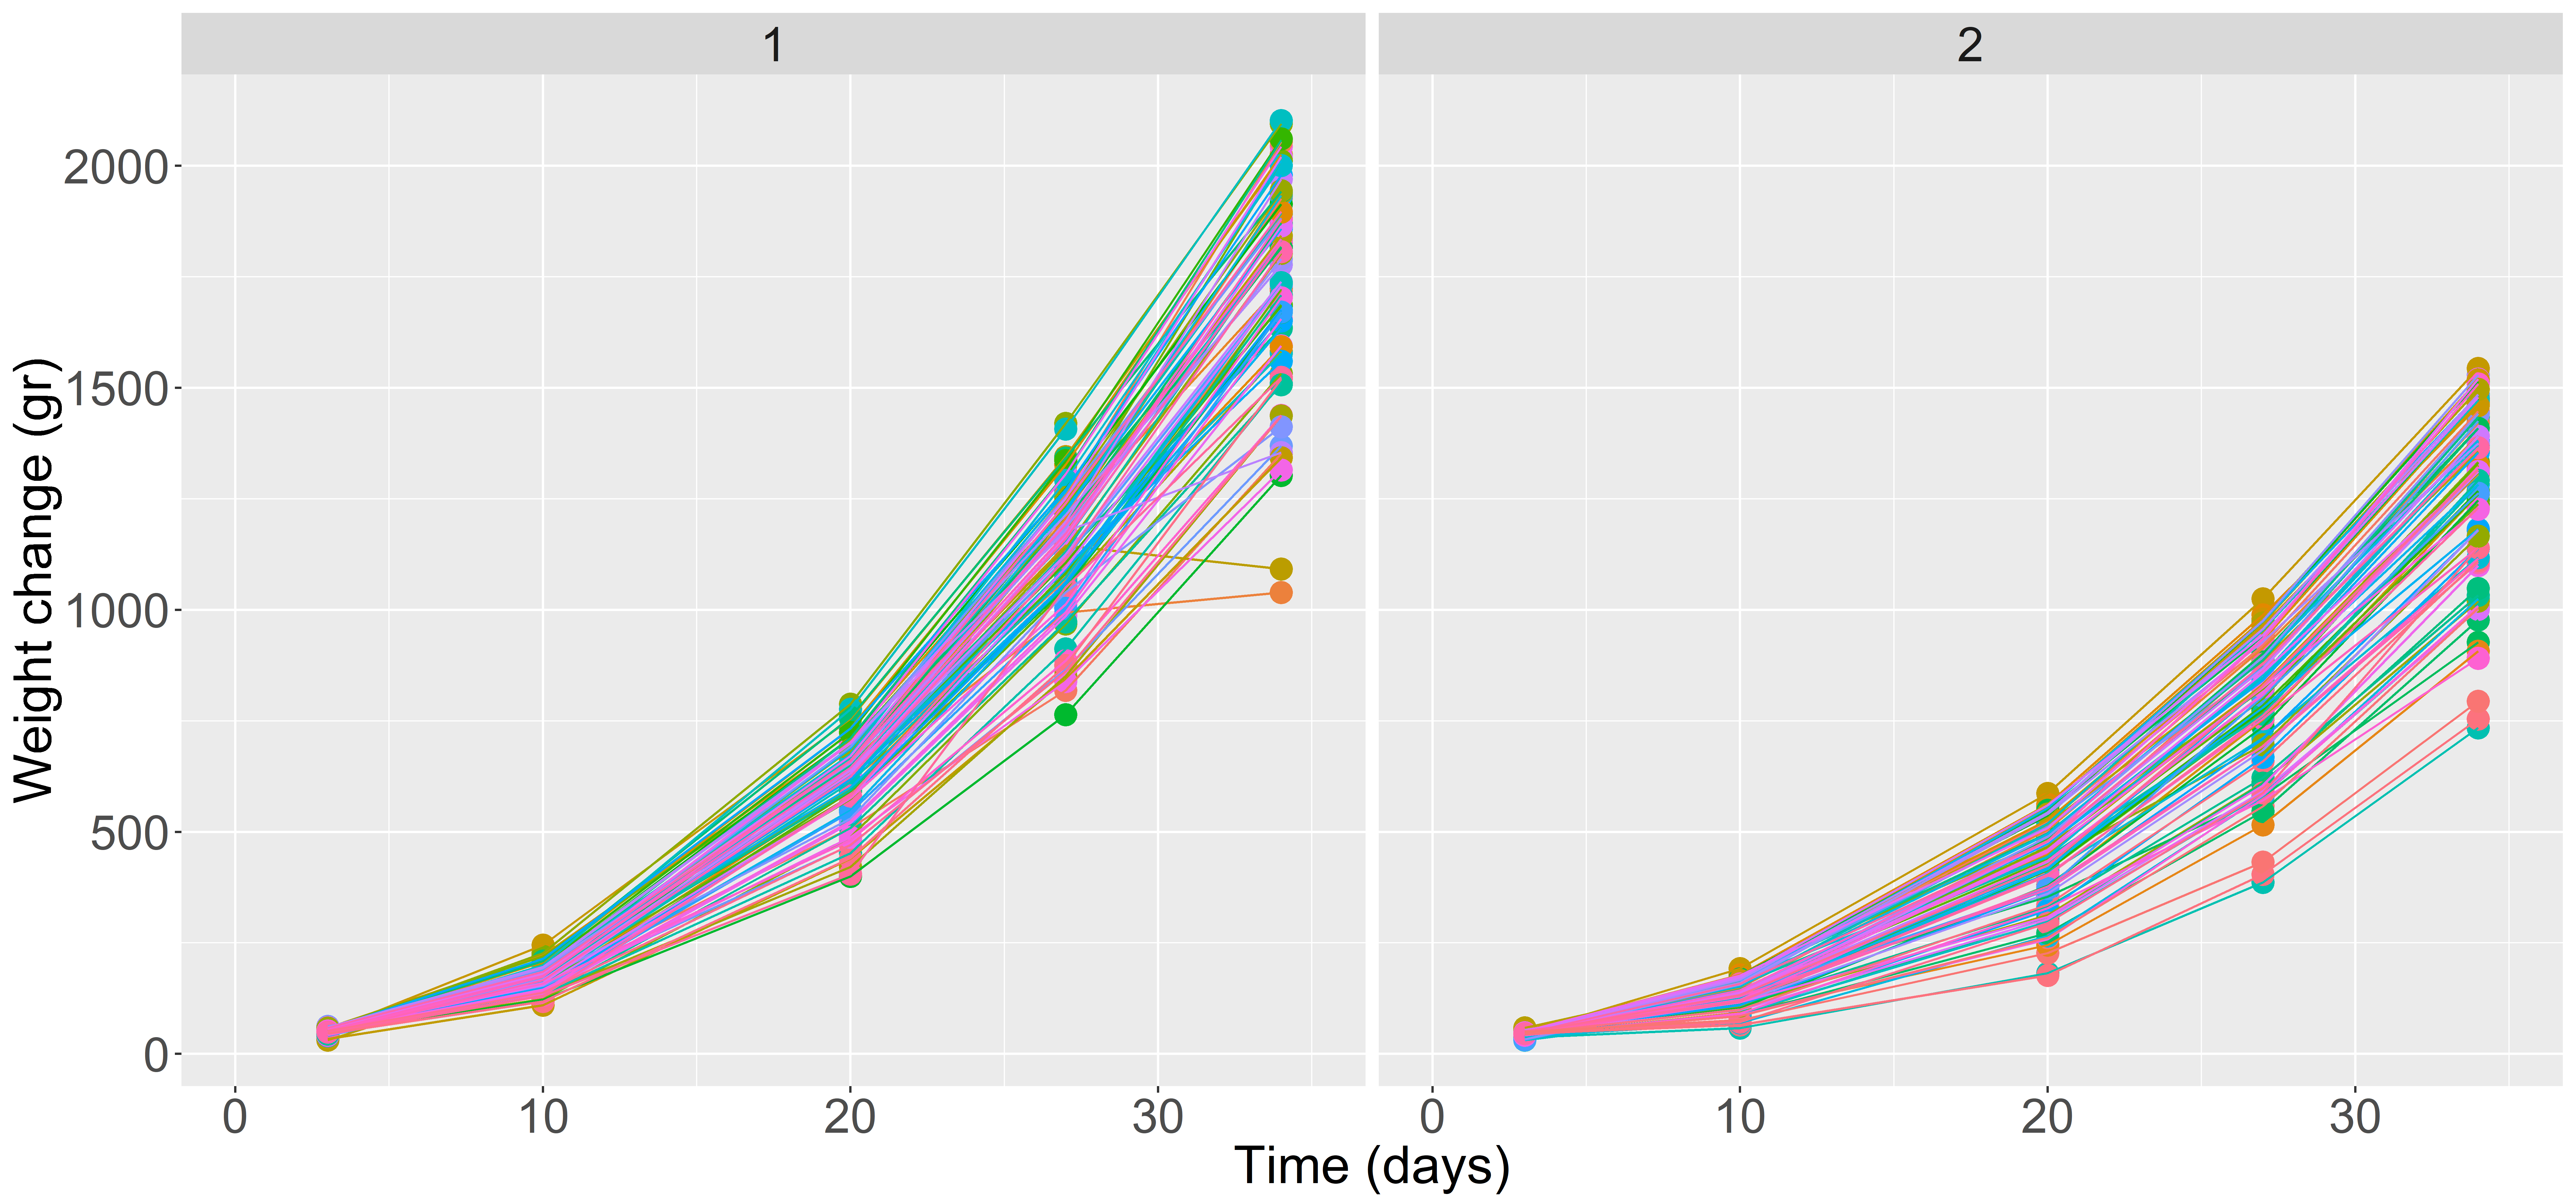
\includegraphics[width =\textwidth]{Weight_Time_profiles.png}
%    \caption{Weight change (gr) over time (days) per chicken}
%    \label{fig:non_transform}
%\end{figure}

In the first part of the study, after some descriptive statistics, we fitted a classical mixed model. We compared the fitted models using a transformed outcome variable and one without transformations. We analyzed the possible interactions and made some conclusions on which group is more likely to experience weight loss. In the second part we decided to use longitudinal models, in order to capture and model in a better way the time dependency structure of the data. 

add for second part smthg 

\section{Classical Mixed Modeling}

The first step we took was to fit a simple classical mixed model. We introduced the following variables as fixed effects: Department, Group and Time. The variable Pen is introduced as random effect, since we assume that there is a certain dependency structure between diseased chicken in the same pen. The variable ID was also introduced as a random effect, and it represents the random chicken effect since repeated measurements on the same chicken are obviously dependent. 
For the variable Time we used a second order polynomial. Higher order polynomial give the approximately the same result, thus we choose the second order polynomial to keep the model as simple as possible, as we can see below(Figure 2).


%\begin{figure}[h!]
%    \centering
%    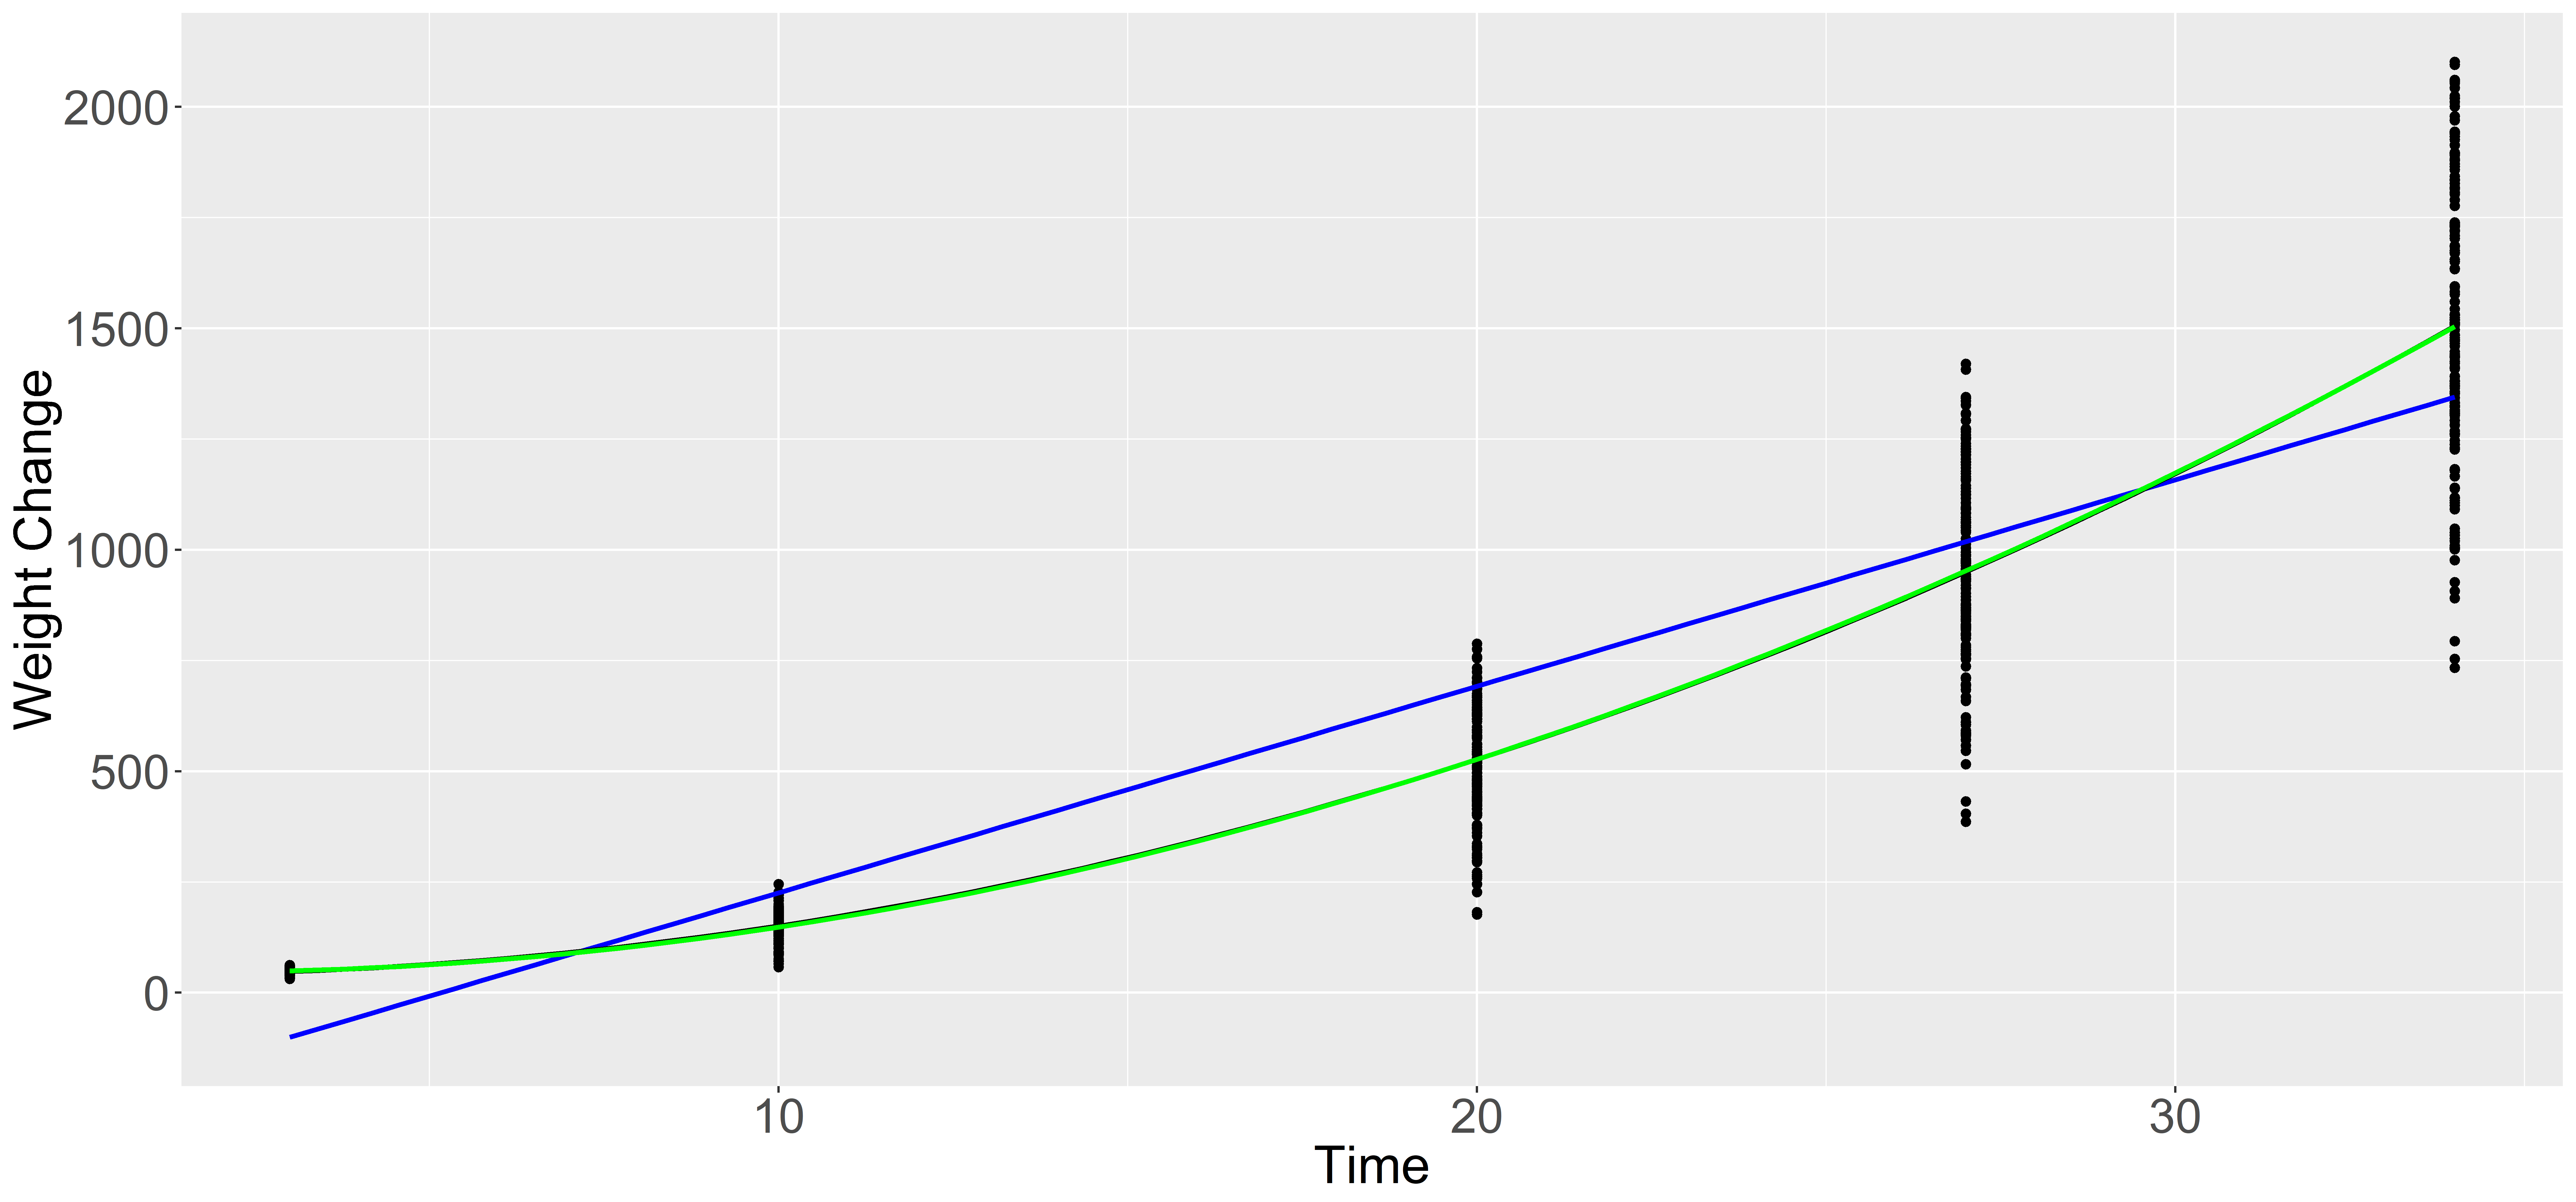
\includegraphics[width=\textwidth]{Fit_poly.png}
%    \caption{Relation between outcome variable and time.
%    (green line second order polynomial)}
%    \label{fig:transform}
%\end{figure}

Initially, we did not apply transformations to the outcome variable and we did not consider interactions. # fix model specification 

\begin{equation}
    y_{ij} =  \beta_0  + \beta_1 \cdot Group_i + \beta_2 \cdot Time_{ij} + \beta_3 \cdot Department_{i} + \beta_4 \cdot Pen  + \varepsilon_{ij}
\end{equation}




The results of the aforementioned model are shown below(Table ...). The model was fitted using REML due to the fact that we have unbalanced data. The tests carried out on the parameters of the model are all significant (considering an $alpha$ = 0.05) expect for the factor Department 34. Having a look at the coefficients we can see that we expect the biggest reduction in weight change for chickens that are in department 23 and part of group 2. Already from this very simple classical mixed model we could think that chickens in Group 2 and Department 23 are more likely to experience weight loss, thus suggesting to take in great consideration this very department and group when deciding to spread MAS disease. 

\begin{table}[ht]
\centering
\caption{Coefficients of model without transformation and interactions}
\begin{tabular}{rrrrrr}
  \hline
 & Estimate & Std. Error & df & t value & Pr($>$$|$t$|$) \\ 
  \hline
(Intercept) & 802.13 & 15.77 & 41.28 & 50.87 & $<$0.001 \\ 
  Department23 & -135.52 & 16.70 & 154.74 & -8.12 & $<$0.001 \\ 
  Department34 & -19.30 & 19.01 & 154.77 & -1.02 & 0.31 \\ 
  Department36 & -46.90 & 16.95 & 154.49 & -2.77 & 0.01 \\ 
  Group2 & -212.57 & 11.94 & 154.71 & -17.80 & 0.00 \\ 
  poly(Time, 2)1 & 14833.43 & 136.44 & 645.59 & 108.72 & $<$0.001 \\ 
  poly(Time, 2)2 & 3724.83 & 136.44 & 645.43 & 27.30 & $<$0.001 \\ 
   \hline
\end{tabular}
\end{table}

From the plot of the residuals against fitted values we can see that there is a pattern in the residuals(Figure...). When comparing the sample quantiles to the theoretical quantiles of a standardized normal distributions we can see how the sample quantiles start to diverge from the theoretical ones. These plots suggest that we have to transform the outcome variable in a certain way, since some of the hypothesis on which linear models are build, residuals normally distributed and constant variance, are not totally respected.
We can also see the dependency from time in the residuals, each batch refers to the 5 different time points (day:3,10,20,27,34)
 


\begin{figure}[ht]%
    \centering
     {{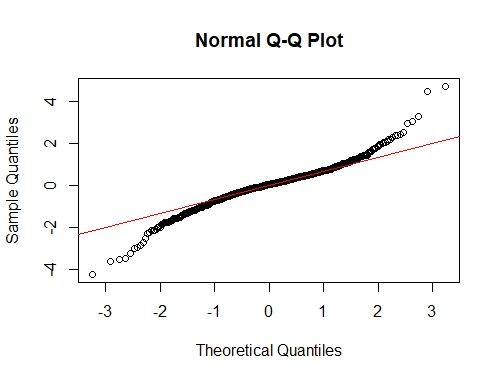
\includegraphics[width=6.5cm]{qqplot_mod_poly_inter_l.jpeg} }}%
    \qquad
     {{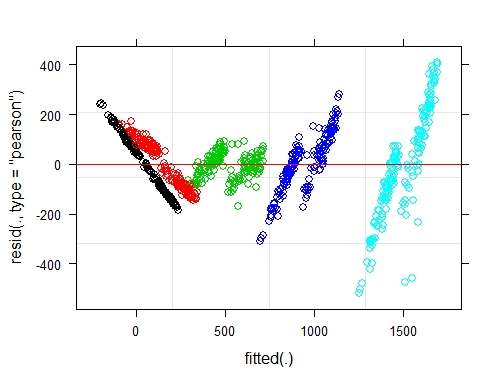
\includegraphics[width=6.5cm]{Resid_mod_poly.jpeg} }}%
    \caption{Quantile plot (left) residuals vs fitted values (right)}%
    \label{fig:example}%
\end{figure}


The solution to fix the problem regarding heteroscedasticity is to transform the outcome variable.
We decided to fit a model with the logarithm transformation of the outcome variable. We choose the logarithm since there is a positive skewness in the distribution of the weight change and also because it keeps the interpretation of the regression coefficients relatively simple.

Below is shown the histogram for the non-transformed outcome variable and the transformed one (Figure...).

We can now see how the Weight Change distribution resembles much more a normal distribution.


%\begin{figure} [h!]
%\centering
%\begin{subfigure}{1\textwidth}
%\centering
%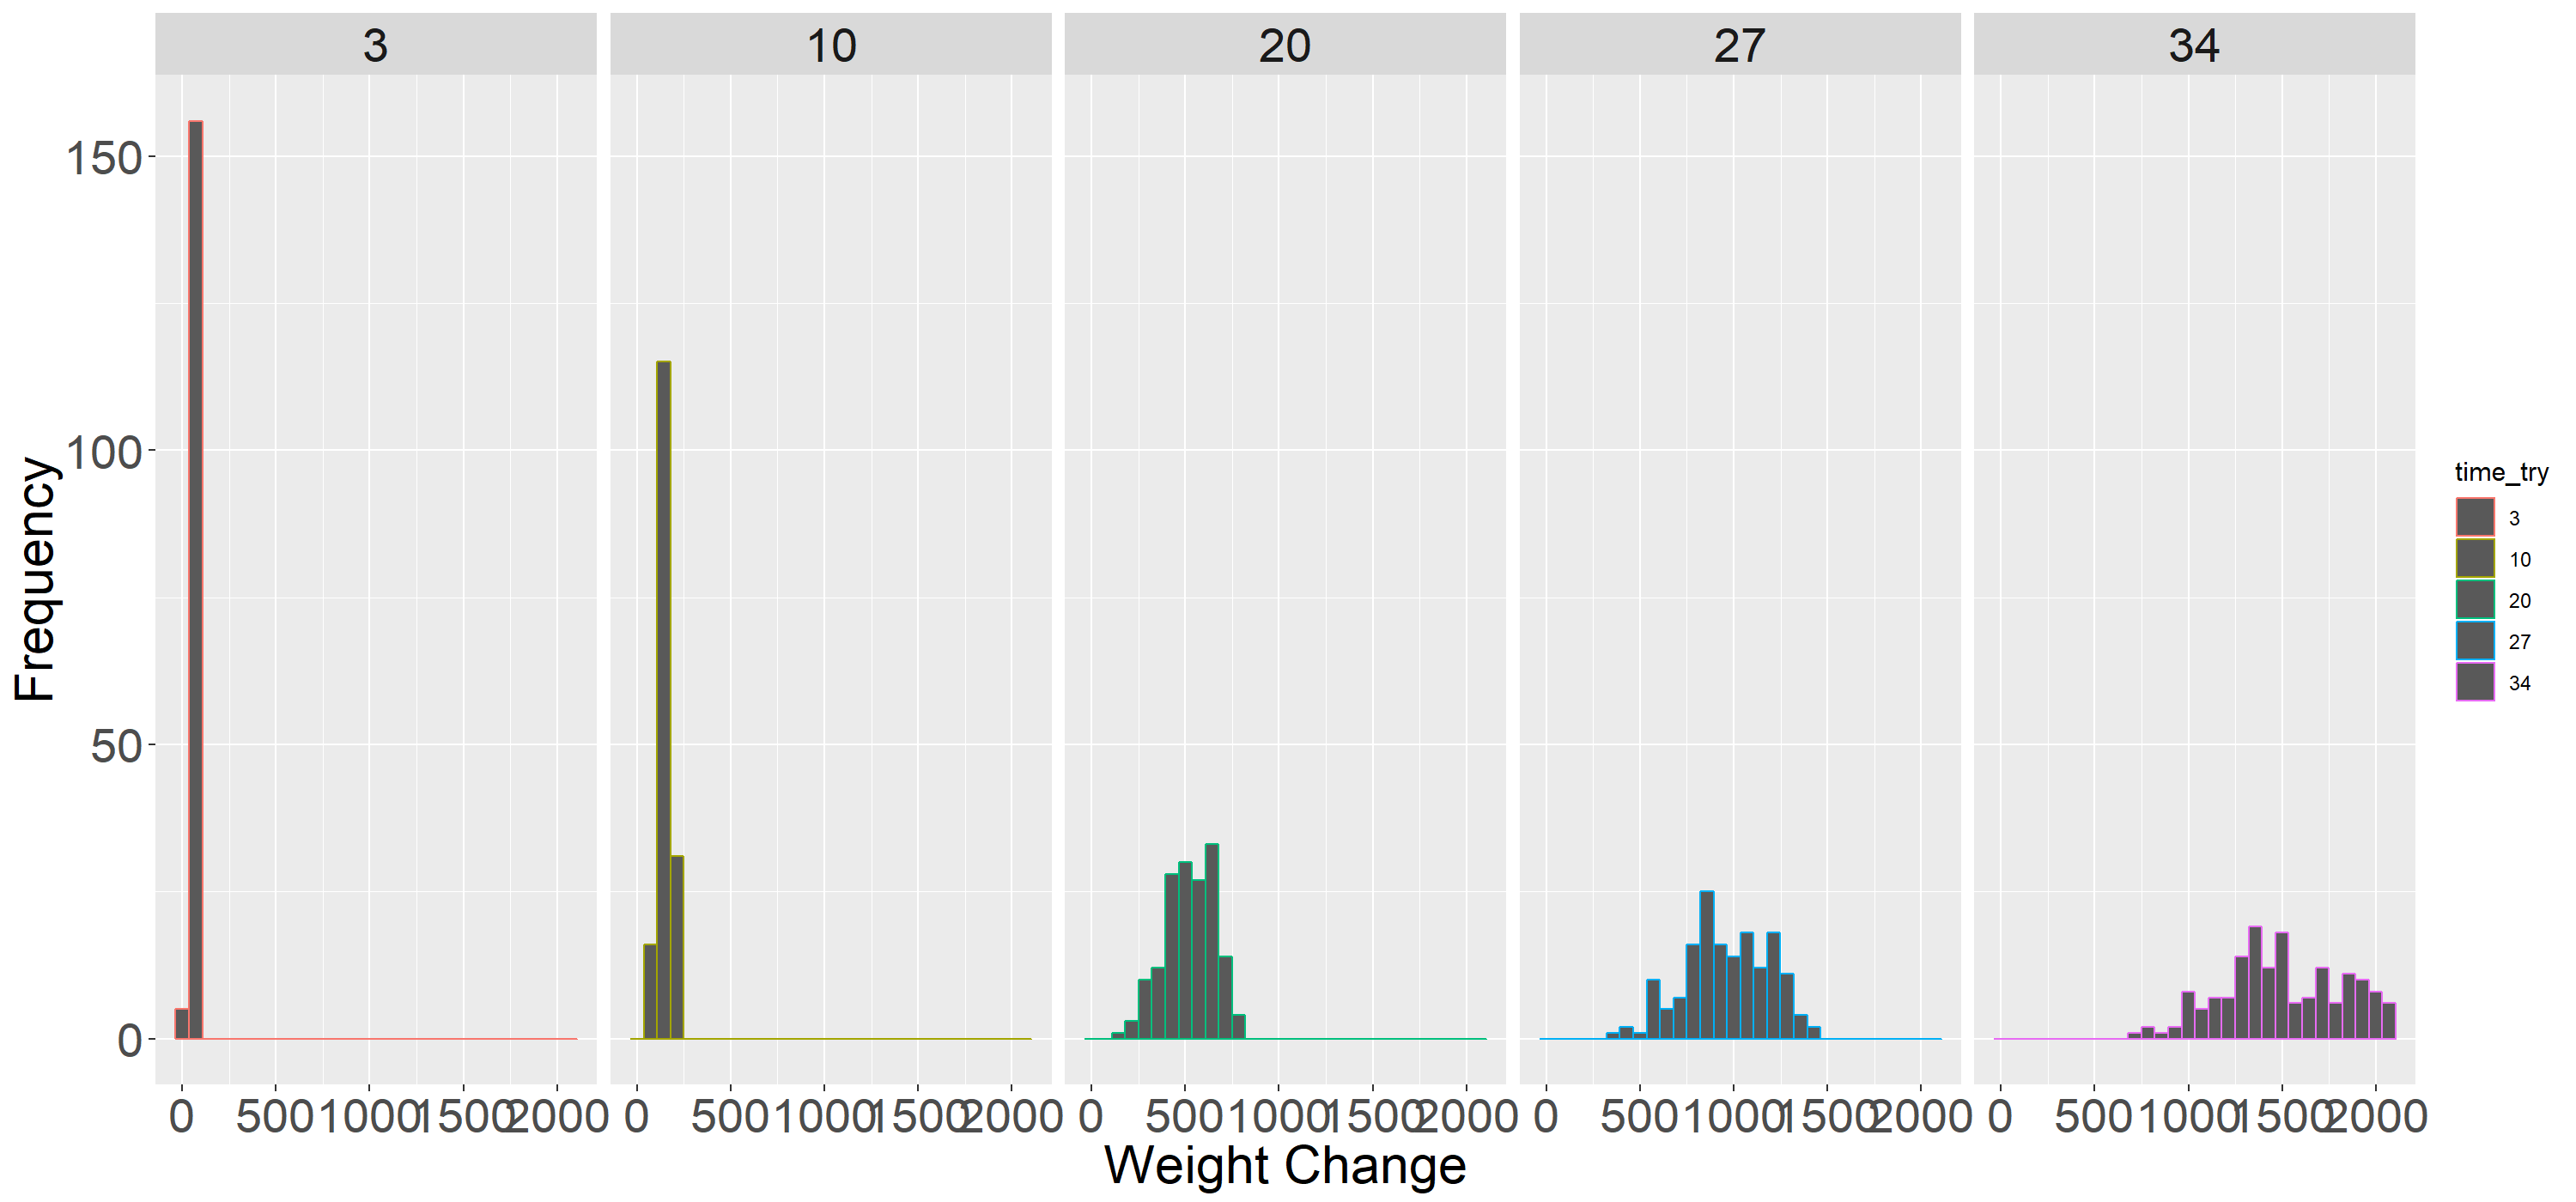
\includegraphics[width=\textwidth]{Histogram_non_trans.png}
%\caption{Histogram per time point without a transformation %of the response}
%\label{fig:hist_non_trans}
%\end{subfigure}
%\begin{subfigure}{1\textwidth}
%\centering
%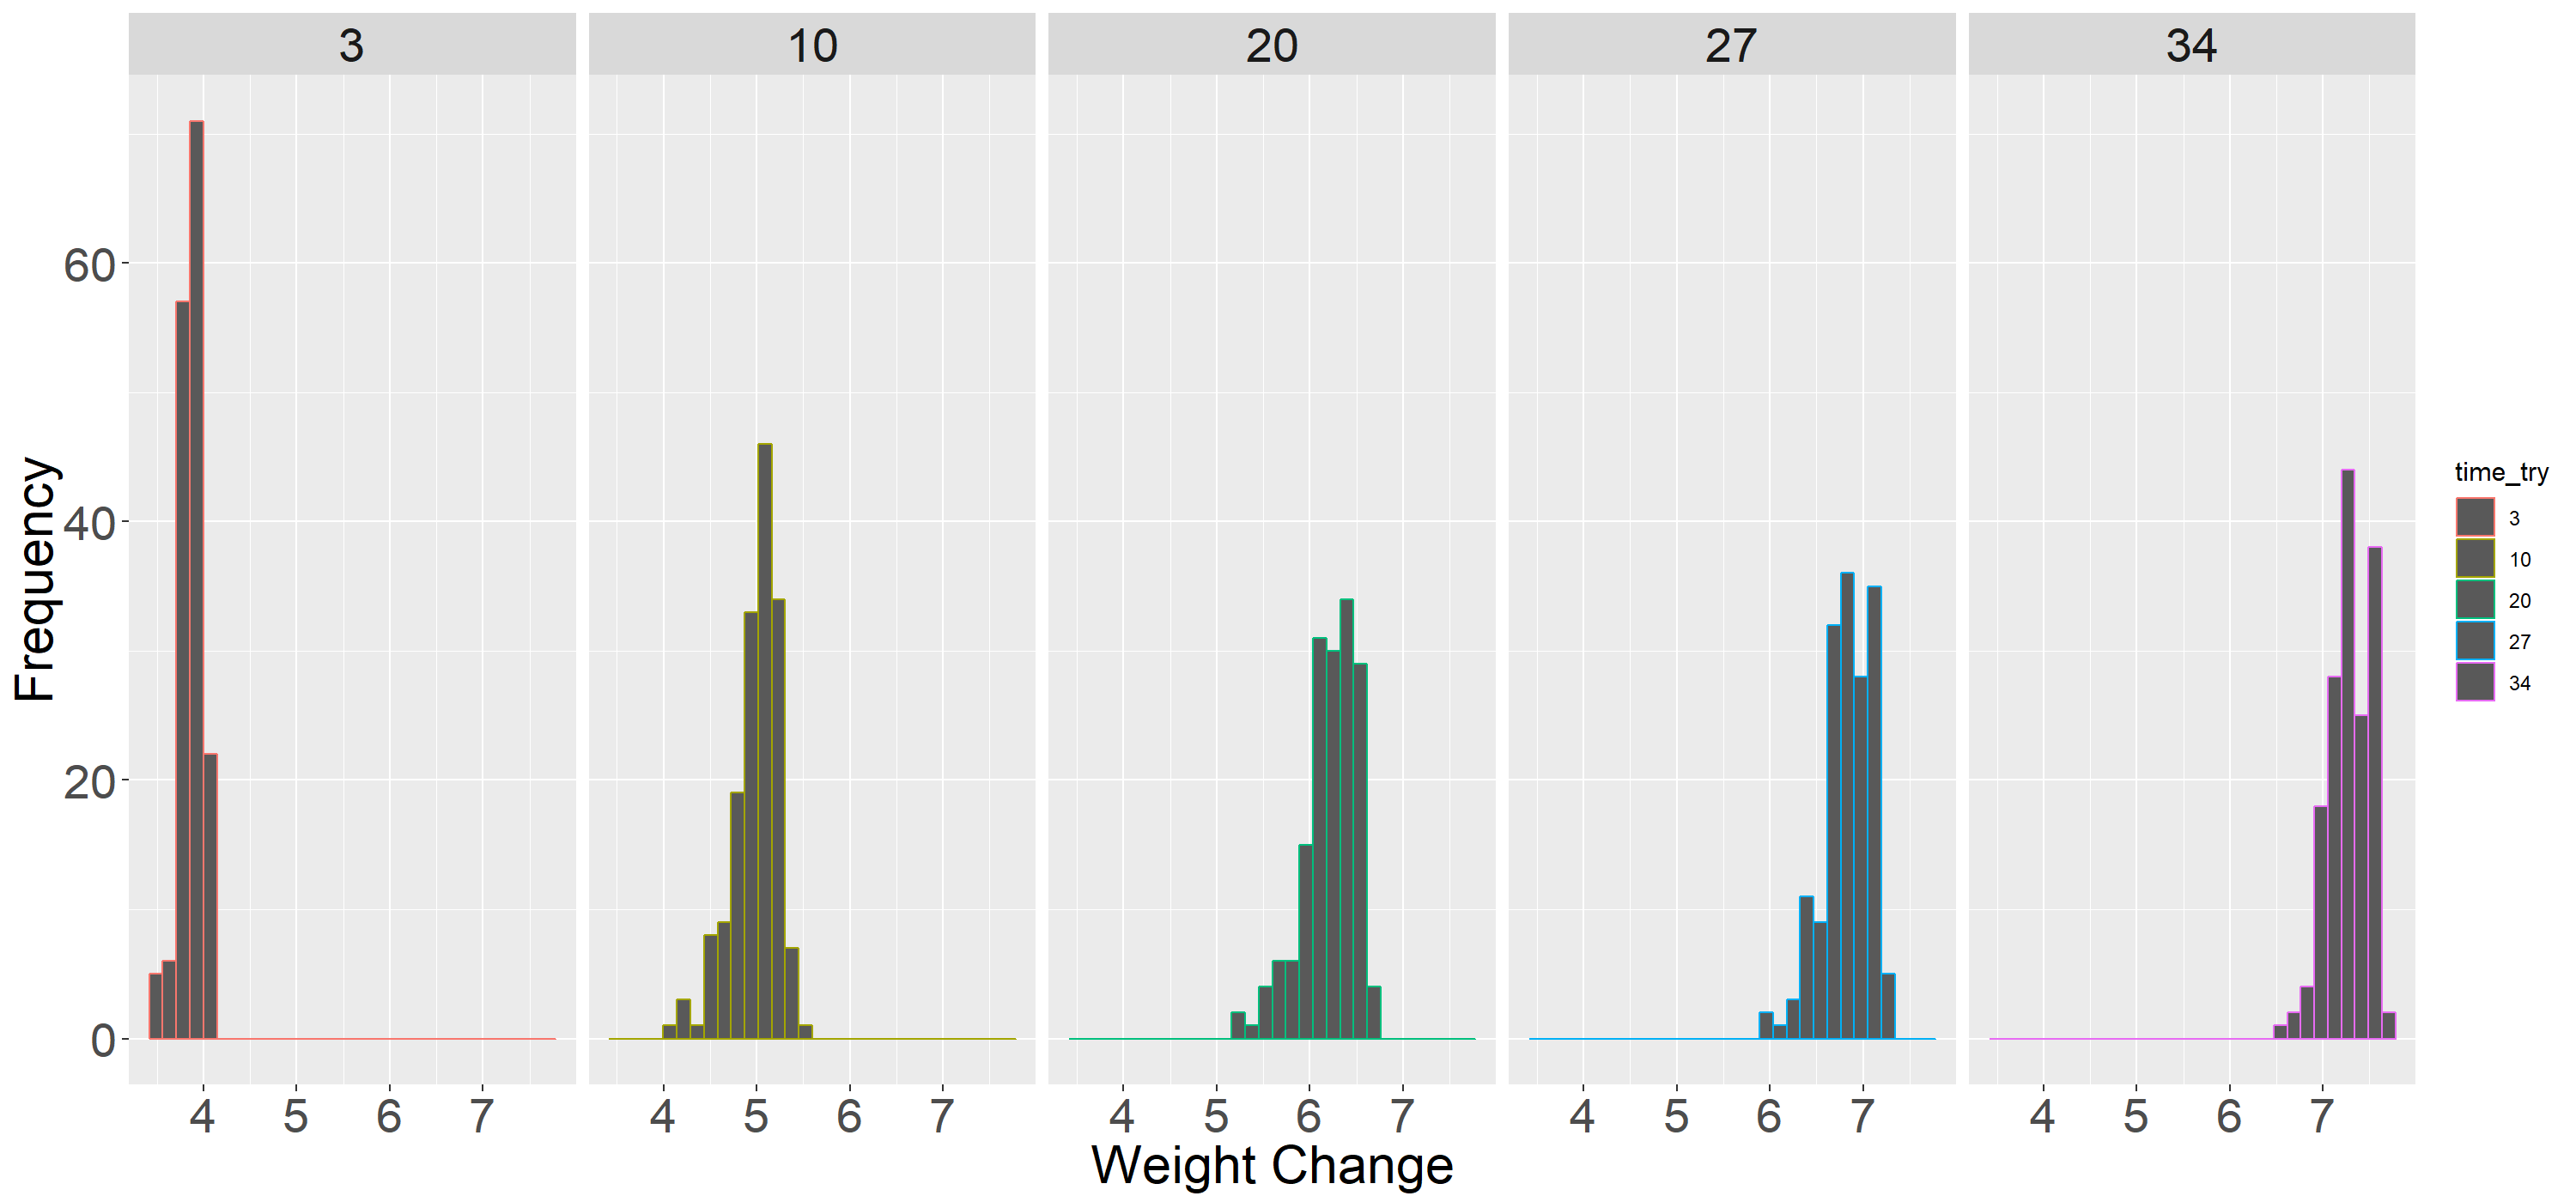
\includegraphics[width = \textwidth]{Histogram_trans.png}
%\caption{Histogram per time points with a log transformation}
%\label{fig:hist_trans}
%\end{subfigure}
%\caption{Histograms with and without a transformation}
%\label{fig:hist}
%\end{figure}


With this in mind, we decided to fit a model with the logarithm transformation of the outcome variable.
We then added the interaction between time and group because it was the only interaction that resulted significant and that might make sense from a logical point of view.
The results are shown below.(Table...)
 
 


\begin{table}[ht]
\centering
\caption{Model with transformation and interaction output}
\begin{tabular}{rrrrrr}
  \hline
 & Estimate & Std. Error & df & t value & Pr($>$$|$t$|$) \\ 
  \hline
(Intercept) & 6.09 & 0.03 & 39.63 & 227.30 & $<$0.001 \\ 
  Department23 & -0.22 & 0.03 & 154.40 & -7.68 & $<$0.001 \\ 
  Department34 & -0.02 & 0.03 & 154.49 & -0.77 & 0.44 \\ 
  Department36 & -0.10 & 0.03 & 154.17 & -3.35 & $<$0.001 \\ 
  Group2 & -0.29 & 0.02 & 154.66 & -14.60 & 0.00 \\ 
  poly(Time, 2)1 & 36.23 & 0.14 & 643.29 & 250.37 & $<$0.001 \\ 
  poly(Time, 2)2 & -6.41 & 0.14 & 643.21 & -44.30 & $<$0.001 \\ 
  Group2:poly(Time, 2)1 & -2.24 & 0.21 & 643.17 & -10.92 & $<$0.001 \\ 
  Group2:poly(Time, 2)2 & 1.95 & 0.21 & 643.13 & 9.48 & $<$0.001 \\ 
   \hline
\end{tabular}
\end{table}


Considering the logarithm transformation we expect more accurate results. The results obtained are similar to the ones obtained by fitting the model without logarithm. Thus, higher weight loss for chickens in Department 23 and in Group 2. 
The plot of the residuals looks much better now, after applying the transformation. The same can be said when comparing with the theoretical quantiles.However, we can still notice a pattern related to the time(even though less accentuated)(Figure...)


\begin{figure}[h!]%
    \centering
     {{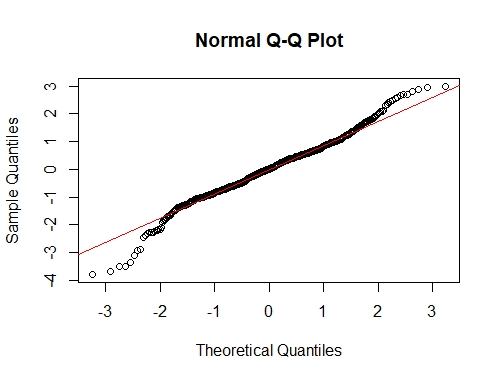
\includegraphics[width=6.5cm]{qqplot_mod_poly.jpeg} }}%
    \qquad
     {{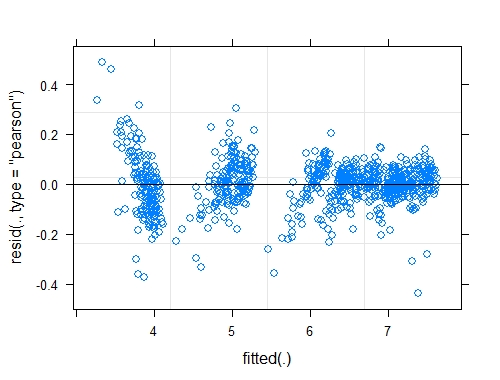
\includegraphics[width=6.5cm]{Resid_mod_poly_inter_l.jpeg} }}%
    \caption{Quantile plot (left) residuals vs fitted values (right)}%
    \label{fig:example}%
\end{figure}
 



We used the Kenward Roger F-test (Table...) to find out if the interaction between group and time is significant. We fitted a model without interaction in order to test it against the one with interaction.

\begin{table}
\begin{tabular}{llllll}
\caption{Kenward Roger F-test}
\hline
       & stat   & ndf  & ddf    & F.scaling & p-value          \\ \hline
F-test & 104.48 & 2.00 & 643.10 & 1         & \textless{}0.001 \\ \hline
       &        &      &        &           &                  \\
       &        &      &        &           &                  \\
       &        &      &        &           &                  \\
       &        &      &        &           &                 
\end{tabular}
\end{table}



Given a significant interaction,we decided to compare the mean differences between the two groups at different time levels. To do so we used a t-test with Satterthwaite's approximation to calculate the (broken) degrees of freedom of the test statistic distribution. We considered the values of Time = 10 and Time = 34.(Table... and ...) 



\begin{table}[h!]
\begin{tabular}{llllll}
\caption{T-test a time point day 34}
\cline{1-4}
                         & stat                    & df     & p-value            &  &  \\ \cline{1-4}
t-test                   & 14.049                  & 156.71 & \textless{}2.2e-16 &  &  \\
                         &                         &        &                    &  &  \\
95\% confidence interval & {[}408.7261,542.4538{]} &        &                    &  &  \\
Mean group 1             & 1737.402                &        &                    &  &  \\
Mean group 2             & 1261.812                &        &                    &  &  \\ \cline{1-4}
\end{tabular}
\end{table}



\begin{table}[h!]
\begin{tabular}{llllll}
\caption{T-test a time point day 10}
\cline{1-4}
                         & stat                    & df     & p-value   &  &  \\ \cline{1-4}
t-test                   & 8.6595                  & 154.85 & 5.82e-15 &  &  \\
                         &                         &        &           &  &  \\
95\% confidence interval & {[}30.29136,4819583{]} &        &           &  &  \\
Mean Group 1             & 170.7561                &        &           &  &  \\
Mean Group 2             & 131.5125                &        &           &  &  \\ \cline{1-4}
\end{tabular}
\end{table}

The more the days the bigger the difference between the two groups. What was found in the previous models is confirmed again by the test, i.e. we expect a bigger weight decrease for chickens in group 2. (the bigger the amount of time from when the disease is injected the bigger the mean loss of weight between the two groups)


The following plot(Figure...) shows the weight change plotted against time for every animal. The transformation affects the variance at each time point, i.e. it gets constant(or close to being it). 
Given the impact of time on the model and the time dependency structure of the data we thought of a better model to analyze this data set. Longitudinal models can be very handy in this case. These very models are helpful to study changes of time and to separate cross-sectional effects from longitudinal effects. In longitudinal models the correlation structure between repeated measurements is modelled via the correlation matrix
In the second part of the case study we analyzed different longitudinal models in order to get a better idea of time effect on weight change, the second plot, for example, might suggest the use of a random intercept model.


%\begin{figure}[ht]
%    \centering
%    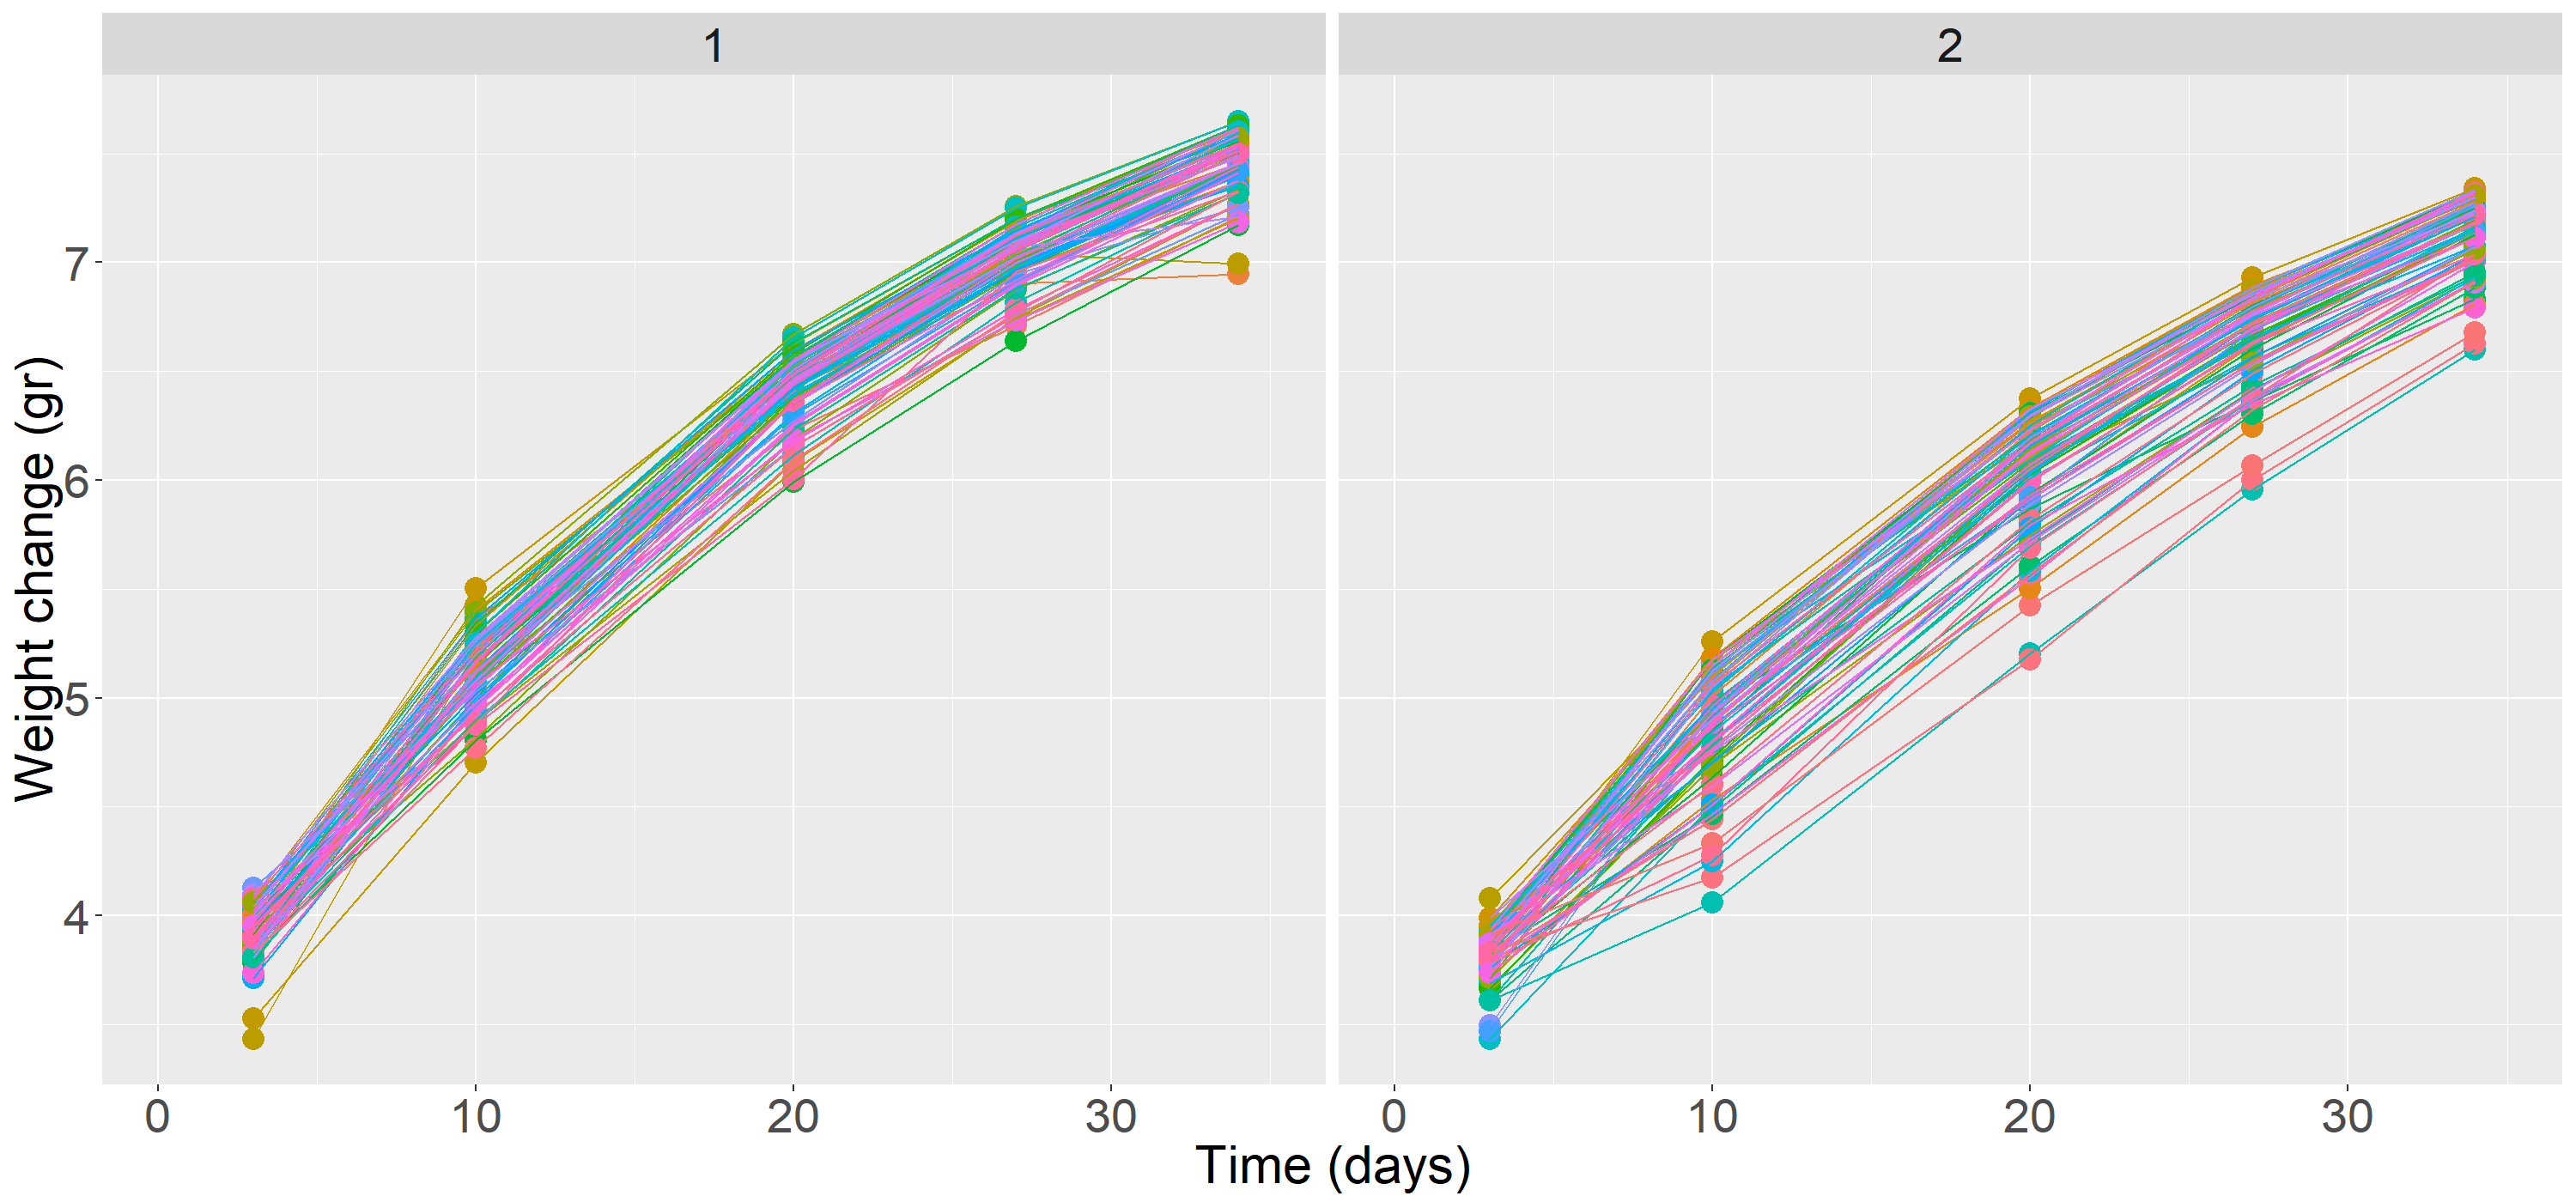
\includegraphics[width =\textwidth]{Weight_Time_profiles_log.png}
%    \caption{Transformed weight change (gr) over time (days) per chicken}
%    \label{fig:non_transform}
%\end{figure}






\section{Longitudinal Mixed Modeling}

A longitudinal model would be a better fitting model, because the measurements are performed over time. This results in dependence between measurements in the same chicken. The dependence can be modeled with a random effects model. This chapter will describe which steps are taken to find the best fitting longitudinal model:
\begin{itemize}
    \item Adding fixed effects
    \item Adding random effects
    \item Adding correlation structures
    \item Visualize final result
\end{itemize}


\subsection{Fixed effects}
As already discussed in the classical mixed model, the response is fitted on a log scale. At first, the minimal model is fitted. The formula is stated below:
\begin{equation}
    log(y_{ij}) =  (\beta_0 + b_0) + \beta_1 \cdot Group_i + \beta_2 \cdot Time_{ij} + \varepsilon_{ij}
\end{equation}

\paragraph{}
Let i = ID, with $i = 1,2,3,\ldots , 162$ and j = Time, with $j = 3,10,\ldots,34$. It is assumed that $E(y_{ij}) = 0$ and $\varepsilon_{ij} \sim N_{n_i}(0, \sum_i)$. Let $b_0$ the random intercept for each ID and $b_0 \sim N(0, D)$. Where D is the appropriate co-variance matrix. $b_0$ and $\varepsilon_{ij}$ are assumed independent.

\paragraph{}
The ML method is used in this part of the analysis. The reason for this is two fold. First, this data set is unbalanced and secondly, because of the comparison of nested models with different $X_i\beta$ parts. The fixed effects are added, one at a time. This eventually least to the maximum model with the interaction between time and group and the different departments. The different nested models are compared to each other with the LRT.

\subsection{Random effects}
As figure \ref{fig:transform} already visualized that the weight of each chicken follows a similar pattern over time, but with different initial weights. Therefore, it hypothesized that a random intercept model is sufficient for this data set. Nonetheless, multiple other random effects are fitted as well. The REML method is used for this part of the analysis, because different random effect structures are compared. The LRT is used the compare models to each other.

\paragraph{}
The model with a random intercept only has a $log(L) = -47.97$ and the model with a random intercept and slope has a $log(L) = -47.60$. However, adding a random intercept and slope resulted in a model with a singular fit. This can indicate that the model is over fitted. In other words, the random effect structure is too complex to be supported by the data. Furthermore, the between group and within group variance is practically zero and the correlation between the random intercept and slope is 1.00.

\paragraph{}
When testing if the variance of a random effect is zero, the null hypothesis is not $\chi^2$ distributed. In this case, the tested null hypothesis is: $H_0: \sigma^2_{int,time} = \sigma^2_{int} = 0$. And the $H_A: \sigma^2_{int,time} > 0$. This results in the following distribution of the LRT under $H_0$:

\begin{equation}\label{eq:mixture}
    0.5 \cdot \chi^2_1 + 0.5 \cdot \chi^2_2
\end{equation}

\paragraph{}
Applying equation \ref{eq:mixture} results in a p-value of 1. It is concluded that a random slope does not improve the model. Next the coefficients and conditional variance-covariance matrix of the random intercept model are visualized. The formula for this final model is:

\begin{equation}
    log(y_{ij}) =  (\beta_0 + b_0) + \beta_1 \cdot Group_i + \beta_2 \cdot Time_{ij} + \beta_3 \cdot Department_{i} + \beta_4 \cdot Time_{ij}\cdot Group_i + \varepsilon_{ij}
\end{equation}
Let i = ID, with $i = 1,2,3,\ldots , 162$ and j = Time, with $j = 3,10,\ldots,34$. It is assumed that $E(y_{ij}) = 0$ and $\varepsilon_{ij} \sim N_{n_i}(0, \sum_i)$. Let $b_0$ the random intercept for each ID and $b_0 \sim N(0, D)$. Where D is the appropriate co-variance matrix. $b_0$ and $\varepsilon_{ij}$ are assumed independent

\begin{table}[ht]
\centering
\caption{Coefficients of random intercept model, fitted with REML}
\begin{tabular}{rrrrrr}
  \hline
 & Value & Std.Error & DF & t-value & p-value \\ 
  \hline
(Intercept) & 3.95 & 0.03 & 645.00 & 123.12 & $<$0.001 \\ 
  Time & 0.11 & 0.00 & 645.00 & 106.94 & $<$0.001 \\ 
  Group2 & -0.16 & 0.04 & 157.00 & -4.65 & $<$0.001 \\ 
  Department\_factor23 & -0.22 & 0.03 & 157.00 & -7.65 & $<$0.001 \\ 
  Department\_factor34 & -0.03 & 0.03 & 157.00 & -0.79 & 0.43 \\ 
  Department\_factor36 & -0.10 & 0.03 & 157.00 & -3.39 & $<$0.001 \\ 
  Time:Group2 & -0.01 & 0.00 & 645.00 & -4.61 & $<$0.001 \\ 
   \hline
\end{tabular}
\label{tab:r1}
\end{table}

\paragraph{}
Table \ref{tab:r1} shows the coefficients of the random intercept model. All coefficients are significant, except for department level 34, with a p-value of 0.43. All coefficients are transformed to the log scale and need to be back transformed for interpretation. Time has a coefficient of 0.11 on the log scale. This translates to $exp(0.11)$ = 1.11 This means that an increase of one unit of time, increases the weight with 11\% in Group 1. Furthermore Group2 has an effect of exp(-0.16) = 0.85. This can be interpreted as a decrease of the mean weight with 15\% at baseline if the chickens are in Group 2. Also the departments have an effect on the weight change of the chickens, $exp(-0.22)=0.80$, $exp(-0.03)=0.97$ and $exp(-0.10)=0.90$, respectively. At last, the change of the weight in Group 2 over time is $exp(-0.16 + -0.01) = 0.84$

\paragraph{}
The amount of variance explained by the random intercept, also called the between-group variance is 0.005. The residual variance, also called the within-group variance is 0.058. This results in an intra-class correlation $\rho$ of 0.08. Table \ref{tab:covar_r1} visualizes the condtional variance-covariance matrix of chicken with ID = 20. The covariance over time is equal to zero.

\begin{table}[h!]
\centering
\caption{Conditional variance-covariance matrix of the random intercept model of ID 20.}
\begin{tabular}{l|lllll}
\hline
           & \textbf{1} & \textbf{2} & \textbf{3} & \textbf{4} & \textbf{5} \\
           \hline
\textbf{1} & 0.05789    & 0          & 0          & 0          & 0           \\
\textbf{2} & 0          & 0.05789    & 0          & 0          & 0          \\
\textbf{3} & 0          & 0          & 0.05789    & 0          & 0          \\
\textbf{4} & 0          & 0          & 0          & 0.05789    & 0          \\
\textbf{5} & 0          & 0          & 0          & 0          & 0.05789  \\
\hline
\end{tabular}
\label{tab:covar_r1}
\end{table}

\begin{figure}
    \centering
    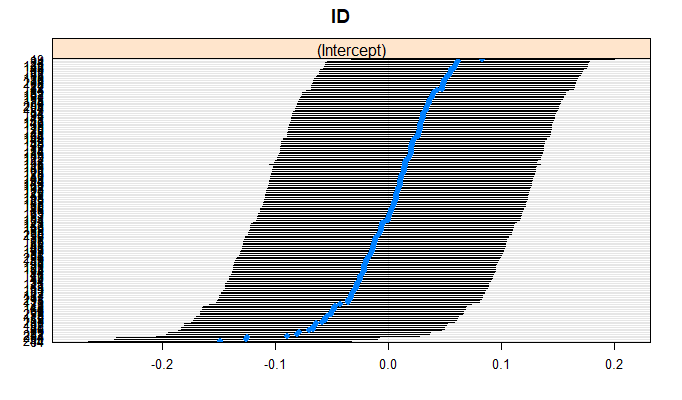
\includegraphics[width =0.7\textwidth]{Random_intercept_r1.png}
    \caption{Estimates (blue dots) and 95 \% confidence interval of the random intercepts for each chicken}
    \label{fig:random_int}
\end{figure}

Figure \ref{fig:random_int} visualizes the estimates of the random intercept. The estimates are in the range from -0.2 till 0.2 and their expected value is close to zero. Each estimate has a 95 \% confidence interval around it. 

\subsection{Correlation structures}
The random intercepts model implies constant variance and constant correlation between any two measurements within subjects. However, this is not always realistic. Therefore, different correlation structures are compared to account for the remaining correlation. In other words, finding the appropriate variance-covariance matrix \textit{D}. The following correlation structures are fitted:
\begin{itemize}
    \item Unstructured correlation, but the algorithm did not convergence 
    \item Compound symmetry correlation (CS), the same correlation over all time points
    \item Autoregressive (AR1) correlation, pairwise correlation decrease with time
    \item Autoregressive-moving average (ARMA) correlation with  autoregressive terms \textit{p} and \textit{q} moving-average terms
\end{itemize}

\begin{table}[h!]
\centering
\caption{Comparison between models with different correlation structures}
\begin{tabular}{llllll}
\hline
                           & \textbf{Model} & \textbf{df} & \textbf{AIC} & \textbf{BIC} & \textbf{Log(L)} \\
                           \hline
\textbf{Random int}        & 1              & 9           & 113.94       & 152.13       & -47.97          \\
\textbf{Random int + CS}   & 2              & 10          & 115.94       & 162.81       & -47.97          \\
\textbf{Random int + AR}   & 3              & 10          & 33.26        & 80.13        & -6.63           \\
\textbf{Random int + ARMA} & 4              & 14          & -449.12      & -383.50      & 238.56  \\
\hline 
\end{tabular}
\label{tab:corr_structures}
\end{table}

\paragraph{}
table \ref{tab:corr_structures} shows the comparison of the different correlation structures performed with the AIC. The AIC uses the Log likelihood and adds a penalty for complexity. A lower AIC generally implies a better fitting model. It is concluded that the random intercept model and ARMA correlation structure is the best fitting model, because its AIC is much lower than for the other models.

\paragraph{}
The ARMA correlation structure has \textit{p=4} auto regressive terms for the fixed effects and \textit{q=1} moving-average term for the random effects. In equation \ref{eq:arma} is \textit{c} a constant and $\varepsilon_t$ is a i.i.d. random variable. $\phi_1,\ldots, \phi_p$ are the fixed stationary variables. The auto regressive model specifies that the output variable depends linearly on its own previous values and the error-term, $\varepsilon_t$. $\theta_1,\ldots,\theta_q$ is the random variables. The moving-average model specifies that the output variable depends linearly on the current $\theta$ and past values of $\varepsilon_{t-1}$.

\begin{equation}\label{eq:arma}
    X_t = c + \varepsilon_t + \sum_{i=1}^p \phi X_{t-i} + \sum_{j=1}^q \theta_j\varepsilon_{t-j}
\end{equation}


\paragraph{}
By applying the ARMA correlation structure, the variance covariance matrix changes as well. The conditional matrix is again shown for ID = 20, see table \ref{tab:covar_arma}

\begin{table}[h]
\centering
\caption{Variance covariance matrix of ID = 20, with ARMA correlation structure}
\begin{tabular}{l|lllll}
\hline 
           & \textbf{1} & \textbf{2} & \textbf{3} & \textbf{4} & \textbf{5} \\
           \hline
\textbf{1} & 0.094      & 0.058      & -0.013     & -0.066     & -0.063     \\
\textbf{2} & 0.058      & 0.094      & 0.058      & -0.013     & -0.066     \\
\textbf{3} & -0.013     & 0.058      & 0.094      & 0.058      & -0.013     \\
\textbf{4} & -0.066     & -0.013     & 0.058      & 0.094      & 0.058      \\
\textbf{5} & -0.063     & -0.066     & -0.013     & 0.058      & 0.094    \\
\hline
\end{tabular}
\label{tab:covar_arma}
\end{table}

\subsection{Final model}
The final model has a random intercept and the ARMA correlation structure. During the analysis, each model is assessed with diagnostic plots. However, only the model diagnostics of the final model with be discussed in this report.


%\begin{figure}
%    \centering
%    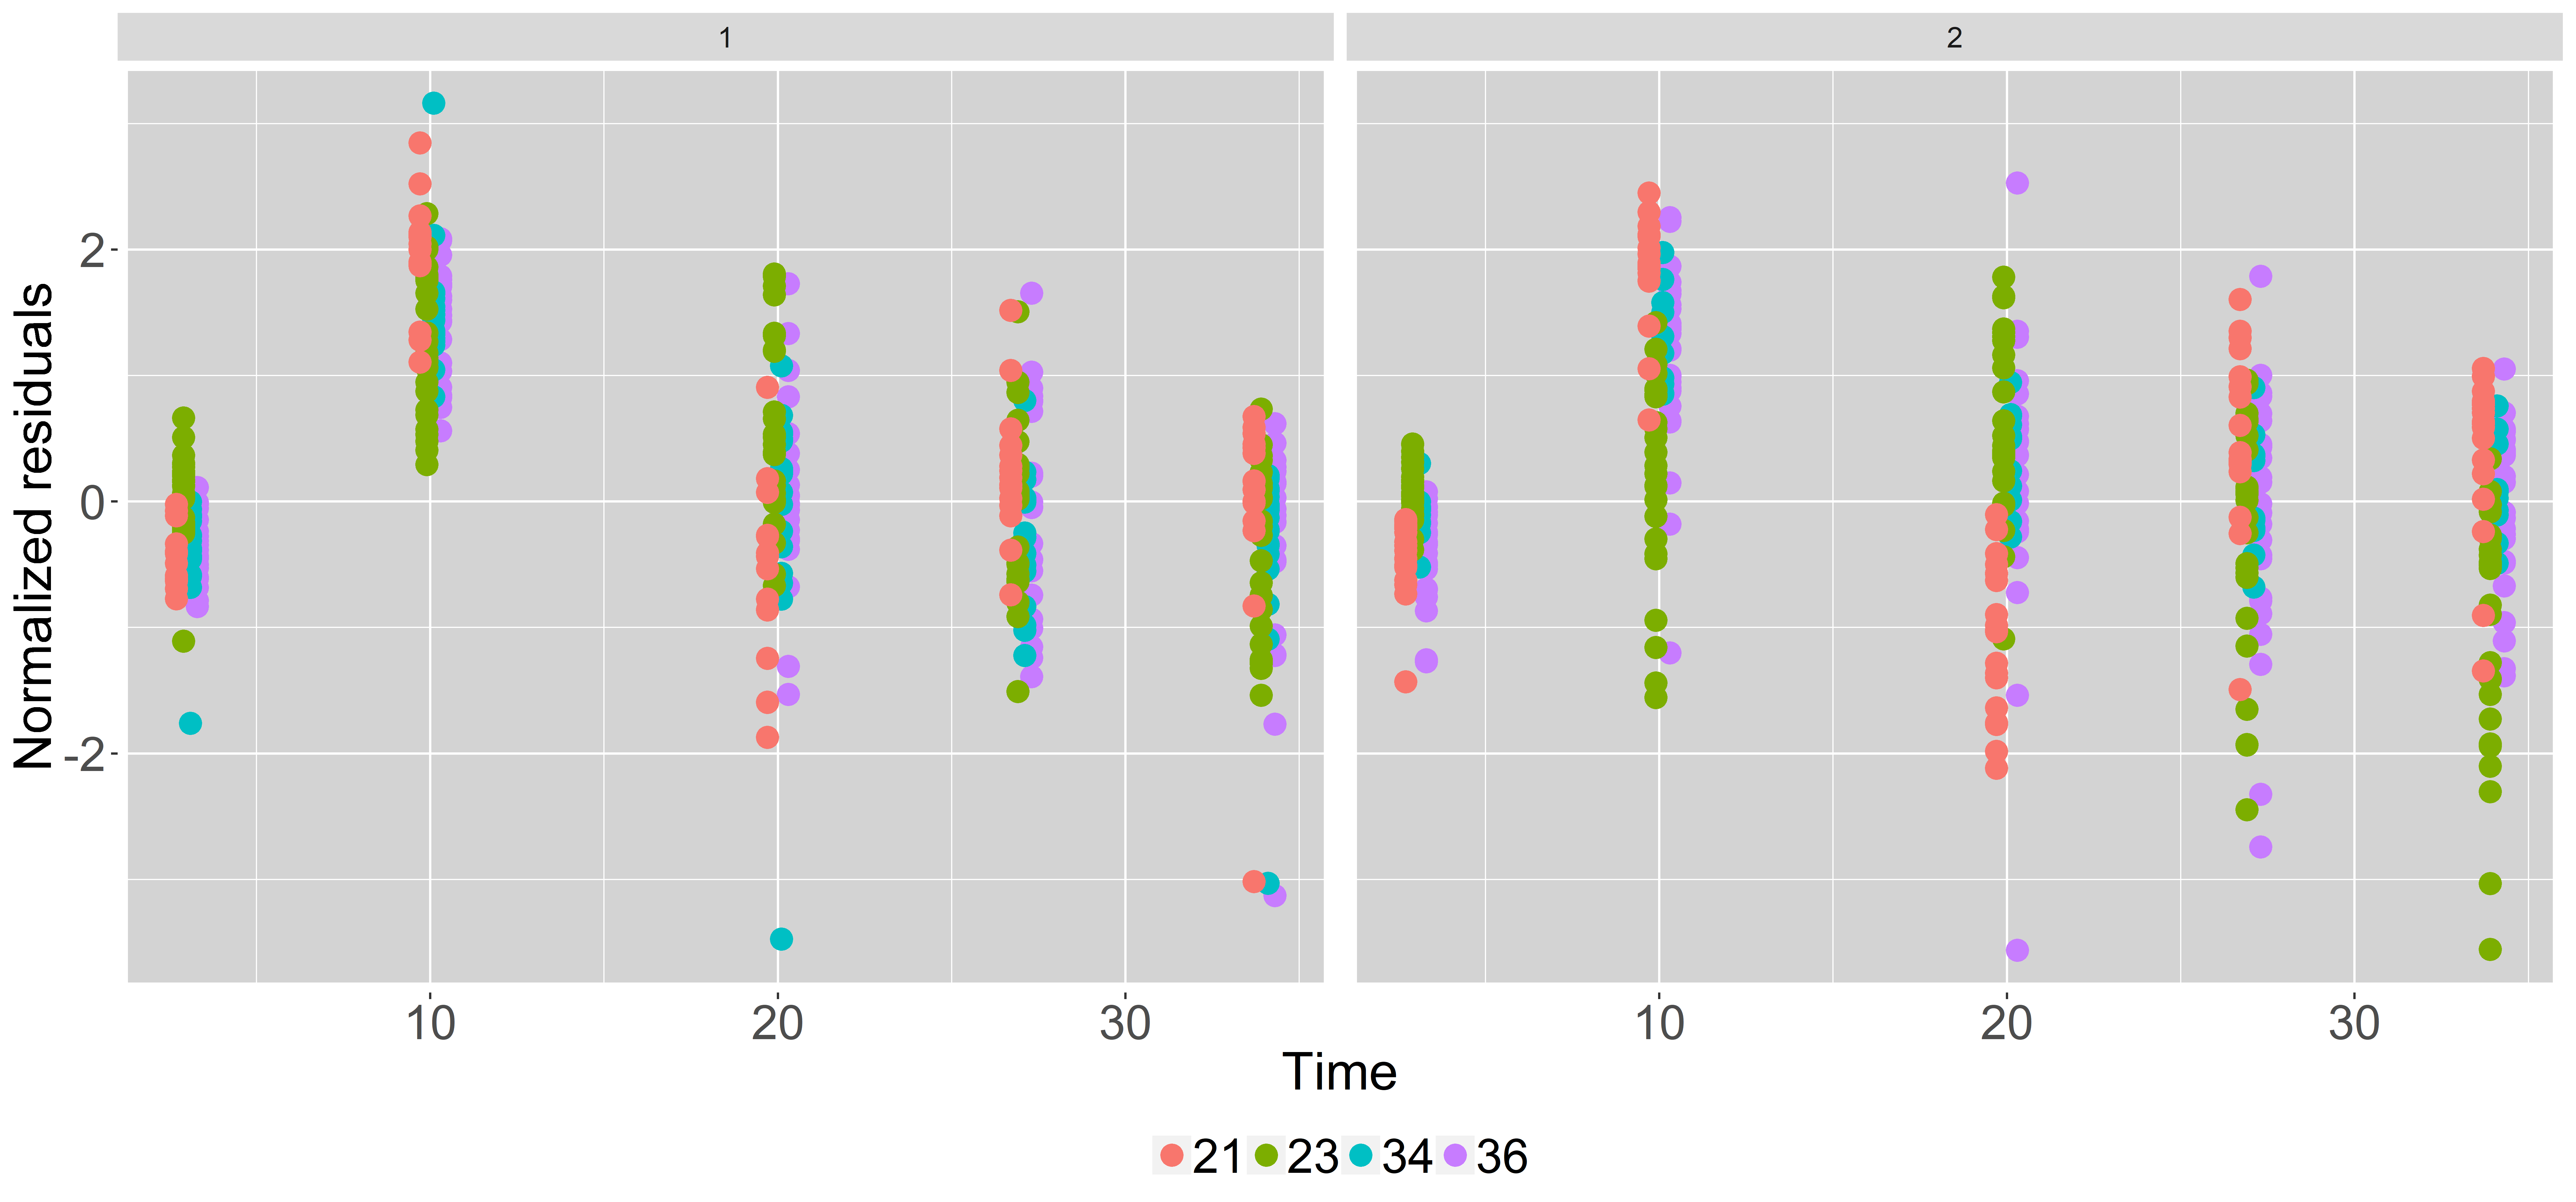
\includegraphics[width = \textwidth]{Residuals_arma.png}
%    \caption{Residuals plotted per time point of the final model. The residuals are colored by department}
%    \label{fig:resid_arma}
%\end{figure}


\begin{table}[ht]
\centering
\caption{Final comparison between group 1 and group 2}
\begin{tabular}{lrrrrrr}
  \hline
Group & Time & emmean & SE & df & lower.CL & upper.CL \\ 
  \hline
1 & 18.8195 & 5.7790 & 0.0128 & 159 & 5.7538 & 5.8043 \\ 
  2 & 18.8195 & 5.5488 & 0.0129 & 159 & 5.5233 & 5.5743 \\ 
   \hline
\end{tabular}
\label{tab:final_result}
\end{table}



\section{Conclusion}
\end{document}
